\documentclass[journal]{IEEEtran}
\usepackage{tikz,adjustbox}
\usepackage{amsmath,amsfonts}
\usepackage{xcolor,graphicx}
\usepackage{amssymb}

\begin{document}

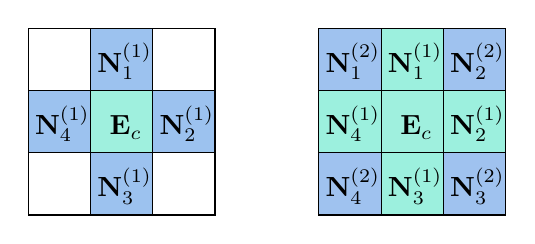
\begin{tikzpicture}[x=0.75pt,y=0.75pt,yscale=-1,xscale=1]

\draw  [draw opacity=0] (211,110) -- (301,110) -- (301,200) -- (211,200) -- cycle ; \draw   (241,110) -- (241,200)(271,110) -- (271,200) ; \draw   (211,140) -- (301,140)(211,170) -- (301,170) ; \draw   (211,110) -- (301,110) -- (301,200) -- (211,200) -- cycle ;
\draw  [fill={rgb, 255:red, 80; green, 227; blue, 194 }  ,fill opacity=0.55 ] (241,140) -- (271,140) -- (271,170) -- (241,170) -- cycle ;
\draw  [fill={rgb, 255:red, 74; green, 144; blue, 226 }  ,fill opacity=0.55 ] (271,140) -- (301,140) -- (301,170) -- (271,170) -- cycle ;
\draw  [fill={rgb, 255:red, 74; green, 144; blue, 226 }  ,fill opacity=0.55 ] (211,140) -- (241,140) -- (241,170) -- (211,170) -- cycle ;
\draw  [fill={rgb, 255:red, 74; green, 144; blue, 226 }  ,fill opacity=0.55 ] (241,110) -- (271,110) -- (271,140) -- (241,140) -- cycle ;
\draw  [fill={rgb, 255:red, 74; green, 144; blue, 226 }  ,fill opacity=0.55 ] (241,170) -- (271,170) -- (271,200) -- (241,200) -- cycle ;
\draw  [draw opacity=0] (351,110) -- (441,110) -- (441,200) -- (351,200) -- cycle ; \draw   (381,110) -- (381,200)(411,110) -- (411,200) ; \draw   (351,140) -- (441,140)(351,170) -- (441,170) ; \draw   (351,110) -- (441,110) -- (441,200) -- (351,200) -- cycle ;
\draw  [fill={rgb, 255:red, 80; green, 227; blue, 194 }  ,fill opacity=0.55 ] (381,140) -- (411,140) -- (411,170) -- (381,170) -- cycle ;
\draw  [fill={rgb, 255:red, 74; green, 227; blue, 194 }  ,fill opacity=0.55 ] (411,140) -- (441,140) -- (441,170) -- (411,170) -- cycle ;
\draw  [fill={rgb, 255:red, 74; green, 227; blue, 194 }  ,fill opacity=0.55 ] (351,140) -- (381,140) -- (381,170) -- (351,170) -- cycle ;
\draw  [fill={rgb, 255:red, 74; green, 227; blue, 194 }  ,fill opacity=0.55 ] (381,110) -- (411,110) -- (411,140) -- (381,140) -- cycle ;
\draw  [fill={rgb, 255:red, 74; green, 227; blue, 194 }  ,fill opacity=0.55 ] (381,170) -- (411,170) -- (411,200) -- (381,200) -- cycle ;
\draw  [fill={rgb, 255:red, 80; green, 144; blue, 226 }  ,fill opacity=0.55 ] (351,110) -- (381,110) -- (381,140) -- (351,140) -- cycle ;
\draw  [fill={rgb, 255:red, 80; green, 144; blue, 226 }  ,fill opacity=0.55 ] (351,170) -- (381,170) -- (381,200) -- (351,200) -- cycle ;
\draw  [fill={rgb, 255:red, 80; green, 144; blue, 226 }  ,fill opacity=0.55 ] (411,170) -- (441,170) -- (441,200) -- (411,200) -- cycle ;
\draw  [fill={rgb, 255:red, 80; green, 144; blue, 226 }  ,fill opacity=0.55 ] (411,110) -- (441,110) -- (441,140) -- (411,140) -- cycle ;

% Text Node
\draw (389,151) node [anchor=north west][inner sep=0.75pt]   [align=left] {$\mathbf{E}_c$};
% Text Node
\draw (383,116) node [anchor=north west][inner sep=0.75pt]   [align=left] {$\mathbf{N}^{(1)}_1$};
% Text Node
\draw (413,146) node [anchor=north west][inner sep=0.75pt]   [align=left] {$\mathbf{N}^{(1)}_2$};
% Text Node
\draw (353,146) node [anchor=north west][inner sep=0.75pt]   [align=left] {$\mathbf{N}^{(1)}_4$};
% Text Node
\draw (249,151) node [anchor=north west][inner sep=0.75pt]   [align=left] {$\mathbf{E}_c$};
% Text Node
\draw (243,116) node [anchor=north west][inner sep=0.75pt]   [align=left] {$\mathbf{N}^{(1)}_1$};
% Text Node
\draw (273,146) node [anchor=north west][inner sep=0.75pt]   [align=left] {$\mathbf{N}^{(1)}_2$};
% Text Node
\draw (243,176) node [anchor=north west][inner sep=0.75pt]   [align=left] {$\mathbf{N}^{(1)}_3$};
% Text Node
\draw (213,146) node [anchor=north west][inner sep=0.75pt]   [align=left] {$\mathbf{N}^{(1)}_4$};
% Text Node
\draw (383,176) node [anchor=north west][inner sep=0.75pt]   [align=left] {$\mathbf{N}^{(1)}_3$};
% Text Node
\draw (413,176) node [anchor=north west][inner sep=0.75pt]   [align=left] {$\mathbf{N}^{(2)}_3$};
% Text Node
\draw (413,116) node [anchor=north west][inner sep=0.75pt]   [align=left] {$\mathbf{N}^{(2)}_2$};
% Text Node
\draw (353,176) node [anchor=north west][inner sep=0.75pt]   [align=left] {$\mathbf{N}^{(2)}_4$};
% Text Node
\draw (353,116) node [anchor=north west][inner sep=0.75pt]   [align=left] {$\mathbf{N}^{(2)}_1$};

\end{tikzpicture}

\end{document}